%! TEX root = ../main.tex
\section{Educación con TIC's}
\label{sec:tics_EDUCACION_TICS}

Las expectativas iniciales acerca del impacto de las \Gls{tic} en la educación
fueron ampliamente superiores a los resultados obtenidos\cite{unesco:ict}. Con
el advenimiento de las computadoras se redujo esta diferencia entre las expectativas 
y lo obtenido, en mayor medida por que se utilizo a las \Gls{tic} en conjunto con 
tecnologías como Internet, y los efectos positivos en la educación fueron aumentando
gradualmente\cite{unesco:ict}.

Una de las principales ventajas de la utilización de las \Gls{tic} en la educación es
su aplicabilidad en áreas como:

\begin{description}

    \item[Nuevos modelos pedagógicos] teorías como el constructivismo moderno
        enfatizan el proceso de como adquirir (aprendizaje) conocimiento y no
        solamente como transmitir el conocimiento en sí (enseñanza).

    \item[Eliminación de distancias] Con la aparición de las computadoras y los satélites, 
        el mundo se ha convertido en una aldea global, y las distancias en cuestiones de
        transmisión de información se han vuelto insignificantes\cite{mohammed2013information}, 
        los medios tradicionales como bibliotecas, o escuelas están limitados a un espacio 
        físico, con el uso de las \Gls{tic}, esta restricción física
        desaparece\cite{tinio:ict}.

    \item[Colaboración distribuida] como consecuencia del punto anterior, los
        alumnos pueden colaborar de manera más sencilla pues no tienen
        limitaciones físicas. Además, los alumnos pueden consultar con expertos
        que están en linea, e incluso tener mentores en linea, estas tutorías
        pueden ser uno a uno, por ejemplo mediante comunicaciones por correo
        electrónico. Además permite la colaboración masiva entre estudiantes de
        intereses comunes, mediante foros y redes sociales\cite{unesco:ict}.

    \item[Motivación para aprender] Las \Gls{tic} tienen un impacto positivo en
	    el proceso de aprendizaje especialmente en lo referente al
	    compromiso con \cite{passey2004motivational,egenfeldt2007third}:
	    
	    \begin{itemize}
	    \item La actividad: a través de estímulos visuales,
	    auditivos, etc.
	    \item La capacidad de investigación: es más fácil acceder a
	    gran cantidad de información bibliográfica.
	    \item La capacidad de escritura y lectura: emitiendo compartir 
	    ideas de manera más legible y mejorarlas iterativamente.
	    \item La capacidad de presentación: es más fácil
	    presentar trabajos profesionalmente a un público
	    mayor.
	    \end{itemize}
	    
    \item[Adquisición de habilidades básicas] las habilidades necesarias para
	    utilizar de manera efectiva las \Gls{tic} se están convirtiendo en
	    una necesidad básica, un aprendizaje guiado por las mismas puede
	    ayudar a una rápida asimilación de los conceptos
        \fixme{relacionados}{Por qué?}.

\end{description}

Uno de los desafíos más importantes que enfrentan las \Gls{tic} para convertirse
en una alternativa viable es la inversión en infraestructura
necesaria\cite{unesco:ict}. 

\subsection{Historia}

\observacion{Por que estos hitos son relevantes, agregar un párrafo que responda}

La historia de las \Gls{tic} en educación comienza con la Universidad Abierta
del Reino Unido\footnote{Open University of United Kingdom} que en 1969 se
establece como la primera institución educativa dedicada a la enseñanza a
distancia utilizando las, para aquel entonces, nuevas
tecnologías\cite{tinio:ict}.

En 1973 Vint Cerf creo el protocolo TCP/IP y es considerado el nacimiento de
Internet\cite{white:ict}, lo que permitió que la información pueda ser
transmitida de manera más sencilla, tiempo después con la aparición de las
computadoras personales en 1977\cite{white:ict}. 
   
\observacion{Conectar más parrafos osino parece que estan citando nomas,
    reordenar}


Otro hito tecnológico se dio en la \Gls{cern} en el año 1989 cuando se concibió
lo que hoy se conoce como \emph{World Wide Web}, permitiendo que los usuarios de
la \emph{Web} puedan compartir archivos mediante un protocolo
estándar\cite{white:ict}. 

\fixme{Con los principales eventos que marcaron la evolución tecnológica de las
    \Gls{tic} en la educación, se divide su historia en cinco partes. Las mismas
    se pueden dividir en dos secciones, las primeras tres corresponden a los
    comienzos y donde los alumnos eran receptores de información, época
    denominada \emph{pull}, y la segunda denominada \emph{push}\cite{white:ict}
    que es aquella donde los alumnos participan de su educación y son creadores
    activos de conocimiento.}{Re-ordenar, llevar más arriba}

\subsubsection{Programación, ejercicios y prácticas}

\observacion{Quizás conviene llevar al final}

Este periodo abarca desde la aparición de las primeras computadoras
personales hasta el final de la década de 1980, se caracterizo por
computadoras muy limitadas, ausencia de interacción multimedia y escasez de
programas especializados. Se enseñaba programación básica\cite{leinonen:ict}, no
por la necesidad de educar programadores, sino por la creencia de que así se
desarrollarían habilidades matemáticas y lógicas en los alumnos. 


\subsubsection{Edutainment}
\todox{Debería ser un nivel más anidado.}

\fixme{En este}{Este cual?} periodo se desarrollaron una gran cantidad de
aplicaciones educativas que más tarde serían conocidas como
\emph{Edutainment}\footnote{Education + Enteirtainment, se traduce como
    educación entretenida}, estas pretendían agregarle entretenimiento a la
educación, se veía al alumno como un receptor pasivo de información que debía
asimilarla, y para aumentar el compromiso, el entretenimiento era
agregado\cite{resnick:2004}.

Esta basado principalmente en la teoría \fixme{del conductismo y el
    cognoscitivismo}{recuerden comentar en el cap1}, se enfoca en juegos
sencillos que transmiten información simple al usuario, siendo este un receptor
pasivo de información, su estructura se basa en un objetivo claro que está
separado de la experiencia educativa\cite{egenfeldt2007third}. Math Blaster
(ver~\ref{fig:math_blaster}) es un \emph{edutainment} donde el alumno debe
responder repetitivamente preguntas aritméticas para obtener municiones, luego
con esas municiones debe completar diferentes misiones en una
nave\cite{bruckman1999can}. Como todas las preguntas se responden mediante un
mecanismo de selección múltiple, y no existe penalización por fallar una
respuesta, rápidamente los alumnos \fixme{seleccionan cualquier opción}{mejorar
    lenguaje}, si no es la correcta, eligen la siguiente, y repiten el proceso
hasta obtener la respuesta correcta, este proceso es conocido como \emph{prueba
    y error sistemático}. 

\begin{figure}[ht!] 
	\centering 
	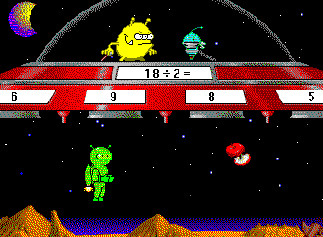
\includegraphics[scale=0.5,natwidth=296,natheight=217]{tics/math_blaster.jpg}
	\caption{Math Blaster, \emph{edutainment} del año 1987}
	\label{fig:math_blaster} 
\end{figure}

Los \emph{edutainment} \fixme{fallaron}{} en enseñar habilidades no triviales, se enfocan
principalmente en enseñar tareas extremadamente repetitivas que no dependen de un
contexto\cite{charsky:2010,egenfeldt2007third,bruckman1999can}, son
excelentes para enseñar a sumar, pero no para aplicar ese conocimiento, analizar
y obtener conclusiones, o evaluar lo que aprendieron.

Las principales causas por del fracaso de los \emph{edutainment} en su intento
de ser una alternativa viable a la educación son según
\cite{egenfeldt2007third}: 

\begin{description}

    \item[Falta de motivación interna] \fixme{la única forma}{mejorar lenguaje}
        que tenían de intentar que el alumno quiera seguir jugando eran las
        recompensas, que eran muy seguidas y fáciles de conseguir.

    \item[Aprendizaje como anexo] el principal objetivo del desarrollo de los
	    \emph{edutainment} eran el de entretener, los objetivos pedagógicos
	    eran agregados al final. Se enviaban informaciones al alumno
	    mediante largos textos que normalmente eran omitidos.
    
    \item[Jugabilidad]\fixme{sencilla}{limitador?} la mayoría eran sencillos
        juegos de arcade, la mayor parte de la interacción eran a través de
        palabras que eran presentadas en forma de selección multiple. 

    \item[Ejercicios de prueba y error sistemáticos] todas las debilidades
	    anteriores se pueden fundamentar en el hecho de que los juegos
	    permitían al alumno intentar varias veces antes de dar una opción
        correcta, sumando \fixme{esto}{quien?} al hecho de que \fixme{los
            mismos}{quien?} no estaban motivados, provocaba que todas las
        opciones sean probadas sin el proceso de reflexión necesario para
        aprender, por ejemplo, varios juegos aritméticos solicitaban pruebas del
        tipo \begin{math}{2+2}\end{math} donde el alumno probaba diferentes
        resultados y luego memorizaba el mismo. Se enseñaba a probar opciones
        sin sentido antes que entender y analizar la experiencia.

\end{description}

\subsubsection{Entrenamiento basado en computadoras}

Cuando aparecieron en el mercado computadoras con multimedia, se argumentó que
los ejercicios de \fixme{la era anterior}{cual era} fallaron en su objetivo de
una educación profunda por que no contenían multimedia\cite{leinonen:ict}, las
aplicaciones eran distribuidas por CD-ROM, y así se actualizaban de manera más
frecuente, y podían contener gran cantidad de contenido multimedia.

Las bases pedagógicas \fixme{de esta}{?} se basada en la capacidad de ciertos
estudiantes de aprender mejor cuando interactúan con contenido multimedia, la
\emph{prueba y error} aún estaban presentes, pero no eran presentados
inmediatamente, sino más bien una vez que el alumno ya debería haber asimilado
los conceptos y funcionaban como pruebas de adquisición de conocimiento. Este
tipo de contenido tampoco logró la enseñanza profunda, solamente fueron
efectivos en el aprendizaje de idiomas, fallando en todos los demás
campos\cite{leinonen:ict}, además los contenidos muchas veces estaban
desactualizados y obtener nuevas versiones no era una tarea sencilla.

Varios gobiernos apoyaron de manera agresiva la introducción de las \Gls{tic} en
educación\cite{mcdougall2006theory} y se realizó un importante avance teórico
con los trabajos sobre el aprendizaje construccionista de Papert y Harel (1991),
y la influencia de las computadoras sobre el aprendizaje y la mente de Marvin
Minksy (1987)~\cite{mcdougall2006theory}.


A comienzos de la decada de 1990, con la popularización de Internet, \fixme{se le vio
    como solución al problema}{Hasta este punto n ose entiende si son areas,
    tipos de enfoque o los dos} de las pocas frecuentes actualizaciones de
aplicaciones educativas, su utilización no tenia bases pedagógicas, más bien se
basaban en la facilidad de distribuir contenido por la \emph{Web}, el principal
inconveniente era la velocidad de Internet, no era suficiente para proveer
entornos ricos en multimedia como lo hacían los CD-ROM\cite{leinonen:ict}.

\begin{figure}[ht!] 
	\centering 
	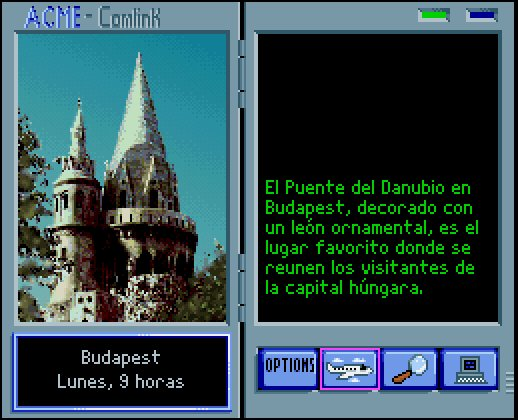
\includegraphics[scale=0.5]{tics/carmen.jpg}
	\caption{Donde en el mundo esta Carmen Sandiego} 
	\label{fig:carmen}
\end{figure}

\fixme{Donde en el mundo esta Carmen Sandiego}{rodear entre comillas}
(ver~\ref{fig:carmen}) es un juego que representa el potencial multimedia de
esta época, el objetivo del juego era detener a una serie de criminales mediante
una serie de pistas que eran provistas en forma de texto\cite{charsky:2010}.
Este exitoso juego demuestra las falencias de esta época, siendo visualmente muy
atractivo, y con contenido multimedia acorde a su tiempo, no era más que prueba
y error, cada nivel del juego podía ser \fixme{completado sin leer el texto que
    contenía la información educativa.}{referencia}

\observacion{Demasiado confuso el formato (osea, como están usando al menos)}


\observacion{Me parece que se mezcla cuestiones técnicas con la pedagogía,
    habrá que separar bien al describir.}

Todos los errores cometidos en la época anterior estaban presentes nuevamente,
no se establecieron marcos teóricos que fundamentasen la utilización de
contenido multimedia, así, se solucionaron los problemas de simplicidad, pero se
demostró que el principal problema era la prueba y error sistemático y sin
sentido\cite{egenfeldt2007third} 

\subsubsection{e-Learning}
\observacion{Esto no debe tener 2.2.X?}

\fixme{ La bases pedagógicas de esta son similares a la era del entrenamiento
    basado en computadoras, se distribuye contenido masivamente a los alumnos, y
    luego, de manera muy discreta se permite a los mismos colaborar, dejando
    siempre en claro que primero se debe asimilar toda la información posible y
    luego relacionarse con los demás\cite{leinonen:ict}. }{difuso}

\emph{E-Learning} se define como la educación y capacitación a través de medios
digitales, incluye todo tipo de medio capaz de distribuir información, puede ser
\fixme{síncrono o asíncrono}{obs: usar términos mas humanos}, y es
particularmente útil para educación a distancia y con horarios flexibles. Se
originó a finales de la década de 1990 y tuvo su apogeo a mediados de la década
del 2000, apoyada por la gran penetración de las \Gls{tic} en la
población\cite{punie:ict}.

Todos los \fixme{paradigmas}{paradigmas, enfoque, etc?, criticar y expliar mejor
    que son  lo} anteriores viven dentro del \emph{e-Learning}, permitiendo
compartir contenido multimedia y realizar pruebas del tipo \emph{prueba-error}. 

\begin{figure}[h] \centering 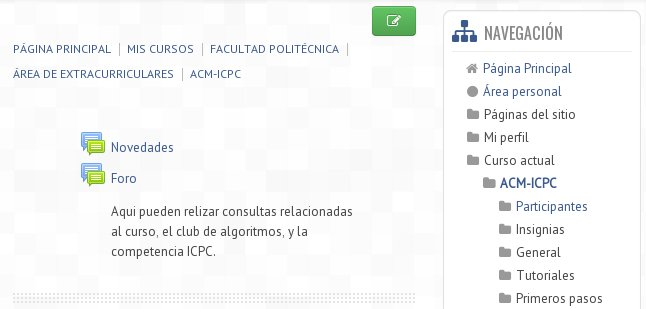
\includegraphics[scale=0.5]{tics/moodle.jpg}
	\caption{Moodle, plataforma de e Learning} \label{fig:moodle}
\end{figure}


\observacion{Tienen que definir mejor como quieren contar esta década? por
    enfoque? es confuso.}

\observacion{AL MARGEN: el trabajo es sobre el análisis y prueba de otro
    tipo/movere(NDT:???) de presentar  contar conocimiento}

La plataforma \emph{Moodle} (ver~\ref{fig:moodle}) cuya primera versión salió en
el 2002, es una de las principales herramientas del \emph{e-Learning} hoy en
día, permite la creación de cursos específicos por materia y sitios
especializados por instituciones académicas\cite{perkins2006using}. 

Si bien en las anteriores épocas, el uso de las \Gls{tic} estaba más orientado
hacia la educación básica y secundaría, el \emph{e-Learning} actualmente es más
utilizado en la educación terciaría\cite{punie:ict}.

La utilización del \emph{e-Learning} tiene varios grados de aplicación en
entornos reales\cite{punie:ict}, que van desde ser simples elementos
complementarios a la clase, como por ejemplo un repositorio para las
diapositivas y otros materiales de clase, hasta cursos completamente en línea,
donde la clase ha sido completamente sustituída.


